\chapter{Prototypdokumentation}
\label{chapter:prototypeDocumentation}

Das vorgehende Kapitel \ref{chapter:systemarchitekur} hat den Systementwurf, die Anforderungen an die Prototypen und das Vorgehen erläutert. Mögliche Probleme und Lösungsansätze wurden aufgegriffen und erläutert. In diesem Kapitel werden die einzelnen Prototypen dokumentiert und die wesentlichen Methoden bezogen auf den Algorithmus aus Kapitel \ref{sec:algorithmus} erläutert. 

In der Dokumentation der Prototypen wird der vollständige Quelltext im Rahmen dieser Arbeit nicht erklärt. Dennoch werden technische Details und wesentliche Methoden speziell erläutert. Um den Schwerpunkt auf den Prototypen zu legen, wird zunächst der Aufbau und die Struktur der einzelnen Java Projekte vorgestellt. Allgemeine Arbeitsschritte und die zusätzlich entwickelten Anwendungen werden zuerst beschrieben. Anschließend werden die Prototypen nacheinander dokumentiert.


\section{Aufbau und Struktur}
\label{sec:prot:aufbauStruktur}

In diesem Kapitel wird der allgemeine Aufbau und die Struktur für die einzelnen Java-Projekte beschrieben. Die implementierten Prototypen bauen auf dieser Struktur auf und haben damit die gleiche Projekt-Basis, sind jedoch unabhängig. Alle Projekte in dieser Arbeit wurden mit Apache Maven erstellt und für die Entwicklungsumgebung \textit{Eclipse} vorbereitet. Da für die Entwicklung der Anwendungen die Versionsverwaltung \textit{git} eingesetzt wird, werden alle implementierten Anwendungen im \textit{git} \textit{repository} \textit{streaming-frameworks} unter dem Verzeichnis \textit{prototype} hinzugefügt. Ausgehend von dem Verzeichnis \textit{prototype} werden verschiedene Verzeichnisse für das \textit{Backend} und der \textit{Visualization} bereitgestellt. Im Unterverzeichnis \textit{prototypes} liegt das \textit{Backend}. Darin sind alle Prototype-Projekte enthalten. Das Unterverzeichnis \textit{helper} besteht aus dem \textit{websocketclient} und den \textit{scriptAndConfigs} Verzeichnis. Der \textit{Websocketclient} unterstützt die Prototypes über den \textit{Broker} in der Weiterleitung der Log-Informationen an die Übersichtsseite. Die erzeugte Bibliothek wird in dem Verzeichnis \textit{protoMavenRepository} hinzugefügt. Die einzelnen Protoypes benötigen dazu einen Konfigurationseintrag unter dem Bereich \textit{dependency} in der Datei \textit{pom.xml}. Das Verzeichnis \textit{scriptAndConfigs} enthält ausführbare Scripte für das Bereitstellen und den Start der Prototypen auf Shell\footnote{Unter Shell wird an dieser Stelle die Kommandoebene unter dem Betriebssystem Linux verstanden.}-Ebene. Der \textit{Broker} vermittelt die WebSocket Nachrichten als Dienst zwischen dem \textit{Backend} und der \textit{Visualization}. Das Unterverzeichnis \textit{webApp} entspricht zuletzt der \textit{Visualization} und enthält die Übersichtsseite für den Apache WebServer zur Darstellung auf dem WebClient. In der Abbildung \ref{fig:systemOverview} werden die einzelnen Prototypen wie der Broker, der WebServer und der WebBrowser dargestellt. Der Broker wird als einzelner Javascript WebSocket-Server implementiert. Damit die Streaming Framework Prototypen nicht über Broker-Systemprozess arbeiten und um den Aufwand gering zu halten, wird jedem Streaming Framework ein Broker in einem eigenen Systemprozess bereitgestellt.

\begin{figure}[htb!]
\centering
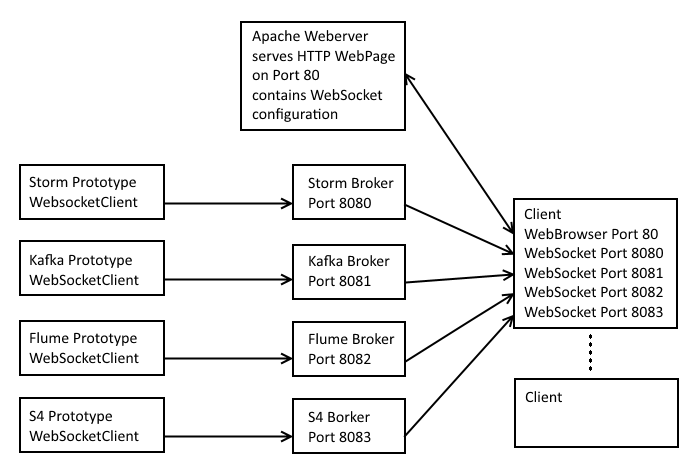
\includegraphics[width=0.85\textwidth]{bilder/SystemOverview.png}
\caption{Systemübersicht
\label{fig:systemOverview}}
\end{figure}

Die Übersichtsseite enthält die Verbindungsinformationen für die Broker. Dadurch können mehrere WebBrowser die Übersichtsseite öffnen und den aktuellen Zustand der Broker beziehen und darstellen. Bei dem erstem Zugriff auf die Übersichtsseite werden alle vier Diagramme der Prototypen noch leer angezeigt. In Abbildung \ref{fig:systemOverviewStart} wird die Übersichtsseite beim ersten Start dargestellt. Im unteren Bereich der Übersichtsseite werden die Informationen und Fehler zu den Verbindungsaufbau zu den Brokern und der Verarbeitung aufgelistet. 

\begin{figure}[htb!]
\centering
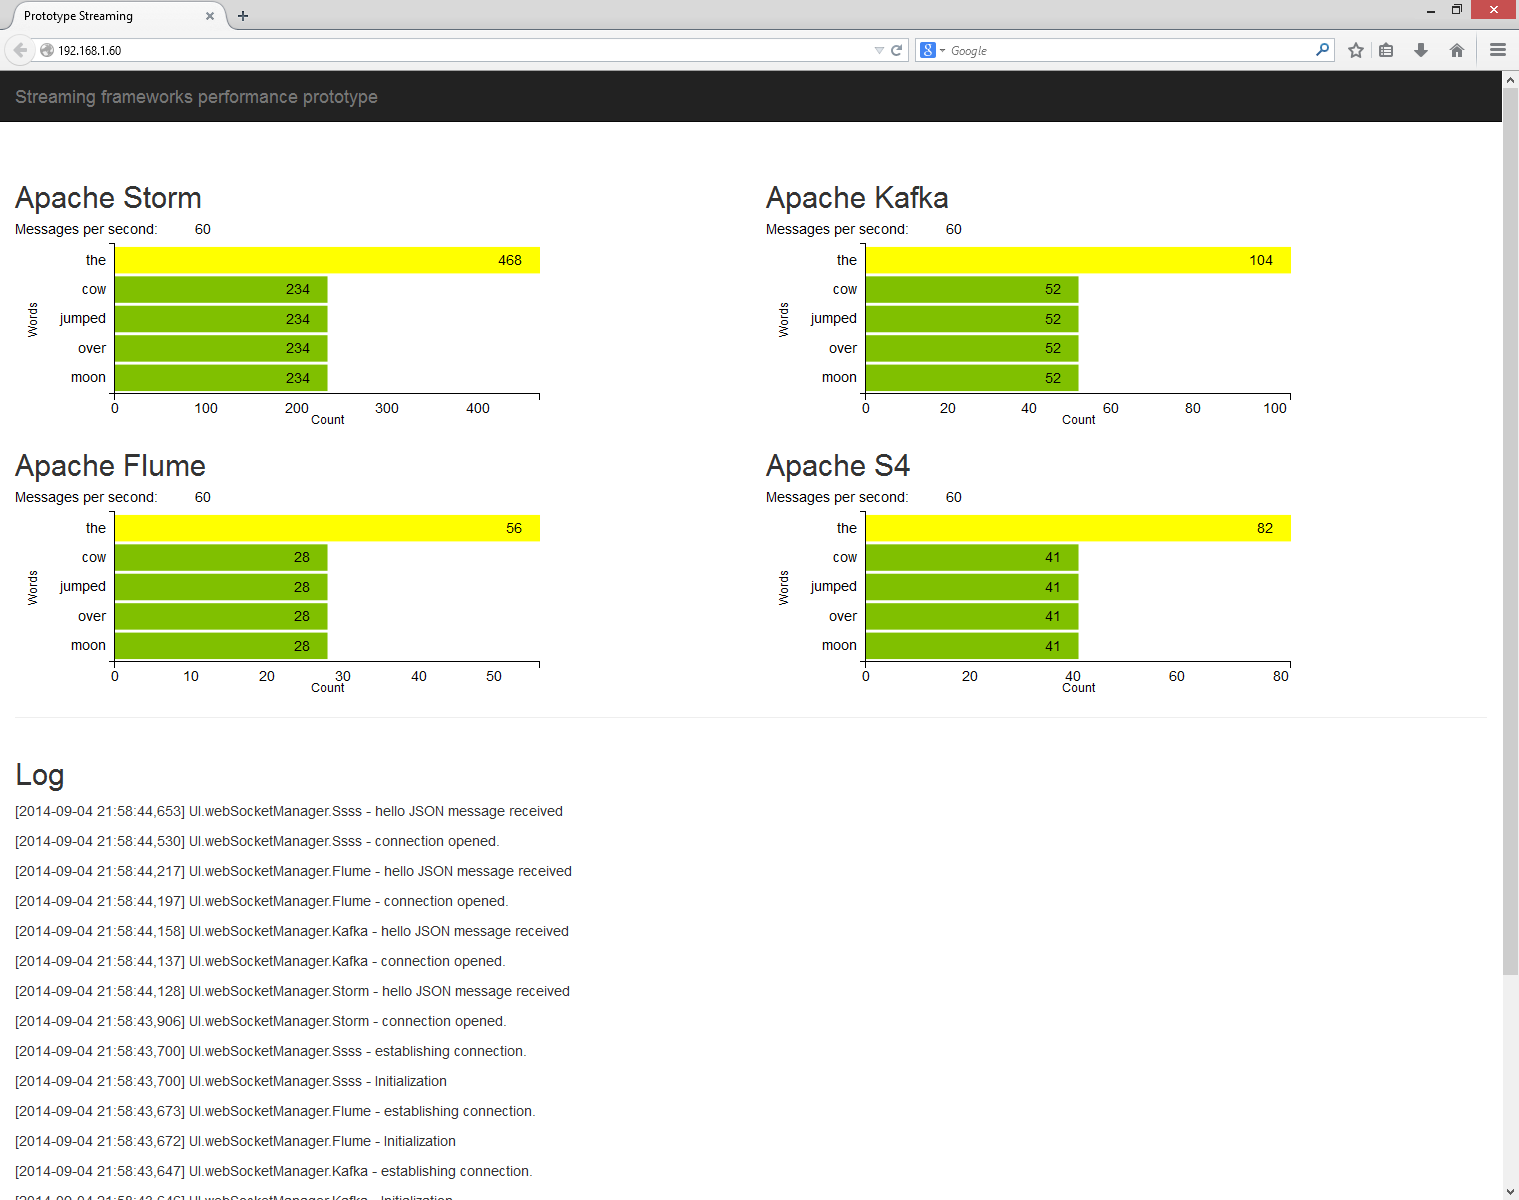
\includegraphics[width=0.85\textwidth]{bilder/PrototypeStreaming001.png}
\caption{Systemübersicht bei erstem Start
\label{fig:systemOverviewStart}}
\end{figure}

Exemplarisch ist der Storm Broker im Listing \ref{lst:stormBroker} dokumentiert. Für die anderen Prototypen muss die Variable \texttt{wsSocketPort} in Zeile 3 im Listing \ref{lst:stormBroker} entsprechend der Portnummer angepasst werden. Für die Ausführung wurden entsprechend in den Unterverzeichnissen lauffähige Broker bereitgestellt.

Die Broker-Systemprozesse werden nach einander in der Shell im Verzeichnis \texttt{prototype/broker} mit folgendem Kommando gestartet:
\begin{verbatim}
>node storm/server.js
>node kafka/server.js
>node flume/server.js
>node s4/server.js
\end{verbatim}

In der Übersichtsseite sind alle Javascripte für die WebSocket Verbindungen und die Darstellung der Log-Information mit der D3-Bibliothek angegeben. Im Listing \ref{lst:graphJs} wird der Quelltext für die D3 Grafik bereitgestellt. Sobald über die Javascript Funktion \texttt{webSocketManager} Nachrichten über den \textit{Trigger} \texttt{messgeIncome} eingehen, kann über den \textit{Javascript Handler} im Listing \ref{lst:mainJs} in Zeile 8 die Methode \texttt{update} aus der D3 Grafik Listing \ref{lst:graphJs} in Zeile 127 aufgerufen werden. Da die Nachrichten vom Prototypen jede Sekunde gesendet werden, wird die D3 Grafik pro Sekunde aktualisiert.

Für die Verbindung zwischen den Prototypen und dem Broker wird im Verzeichnis \texttt{prototype /helper/websocketclient} Java ein Projekt \texttt{websocketclient} bereitgestellt. In den Prototypen wird das Java Archiv referenziert und 
die Instanz für den WebsocketClient über die Factory Klasse mit der richtigen Konfiguration zurückgegeben. In Listing \ref{lst:WebSocketClientFactory} wird über die Methode \texttt{getInstance()} in Zeile 10 die Rückgabe der Instanz für den WebSocketClient gezeigt.

Allgemein werden die Prototypen im Verzeichnis \texttt{target} mit Apache Maven mit folgendem Kommando erzeugt:
\begin{verbatim}
>mvn package
\end{verbatim}

Allerdings müssen für den Prototypen Apache S4 jeweils eigene Java Archive für die einzelnen Variationen erstellt werden. Die folgende Kommandos erzeugen die einzelnen Variationen:
\begin{verbatim}
>mvn package -P intProducer
>mvn package -P intConsumer
>mvn package -P wordCountProducer
>mvn package -P wordCountConsumer
\end{verbatim}

Nachdem die allgemeinen Werkzeuge vorgestellt wurden, werden als nächstes die Prototypen dokumentiert.


\section{Prototype Apache Storm}
\label{sec:prot:storm}

Im Kapitel zuvor wurden notwendige Werkzeuge für die Entwicklung der Prototypen vorgestellt. In diesem Kapitel wird der Prototyp Storm beschrieben. 

Im Listing \ref{lst:stormTopologyWordCount} wird ein Auszug des Storm Prototypen dargestellt. Eine Instanz vom \texttt{TopologyBuilder} wird erzeugt, mit spezifischen Storm-Primitiven konfiguriert und mit der Methode \texttt{submitTopology} in Zeile 15 in das Storm Cluster bereitgestellt. Das Einlesen und teilen des Textes wird in der Klasse \texttt{WordGeneratorSpout} dauerhaft ausgeführt und über \texttt{Tupel}, einem Storm-Datentyp weitergegeben. In der Klasse \texttt{CountPerSecondBolt} werden die Worte aufgenommen, gezählt und pro Sekunde in einem \texttt{Tupel} formatiert weitergegeben. In den Klassen \texttt{PrintBolt} und \texttt{WebSocketBolt} werden jeweils die Log-Information an das Logging-Framework \textit{log4j} und an den Storm-\textit{Broker} weitergegeben. Verbunden werden der \texttt{Spout} und die \texttt{Bolts} über die eindeutigen Namen beim zuweisen der Spouts und Bolts in der Topology, wie zum Beispiel in Zeile 2 \textit{wordGenerator}. Weiterhin wird bei der Konfiguration des \texttt{Bolt} \texttt{CountPerSecondBolt} ein \texttt{fieldsGrouping} auf den Schlüssel \textit{word} gruppiert. Bei den anderen \texttt{Bolts} und dem \texttt{Spout} wird standardmäßig ein \texttt{shuffleGrouping} eingesetzt. Dabei werden die eintreffenden \texttt{Tupel} gleichmäßig über die \texttt{Tasks} im Storm Cluster verteilt verarbeitet.

\lstinputlisting[language=Java,label=lst:stormTopologyWordCount, caption=Java Prototype Storm App Word Counter]{anhangQuelltext/AppWordCounter.java}

Der \textit{Counter} für die konstante Dimension von Werten ist in der Klasse \texttt{AppIntegerCounter} implementiert. Die Implementierung gleicht der Implementierung der variablen Dimension von Werten mit der Klasse \texttt{AppWordCounter}. Anstelle vom Einlesen einer Textdatei werden \texttt{Bytes} von konstanter Größe mit der Dimension 100 in der Klasse \texttt{IntegerGeneratorSpout} eingelesen. Weiterhin wird die Log-Information nur an das Logging-Framework ausgegeben. In Listing \ref{lst:stormTopologyIntegerCount} wird ein Auszug der Klasse \texttt{AppIntegerCounter} dargestellt.

\lstinputlisting[language=Java,label=lst:stormTopologyIntegerCount, caption=Java Prototype Storm App mit konstanter Dimension]{anhangQuelltext/AppIntegerCounter.java}

Die Topologien werden in Storm mit den Scripten \texttt{deployInteger.sh} und \texttt{deployWord.sh} bereitgestellt. Das nächste Kapitel dokumentiert den Prototyp zu Apache Kafka.


\section{Prototype Apache Kafka}
\label{sec:prot:kafka}

In Apache Kafka wird allgemein ein \texttt{KafkaProducer} instanziiert, ein \texttt{Producer} geholt, Daten in einem \texttt{KeyedMessage} verpackt und mit der Methode \texttt{send} aus \texttt{Producer}-Instanz verschickt. In Listing \ref{lst:kafkaWordCountProducer} wird in Zeile 4 ein \texttt{Producer} aus dem \texttt{KafkaProducer} geholt. In Zeile 31 wird ein Wort in einem \texttt{KeyedMessage} verpackt und in Zeile 33 mit der Methode \texttt{send} verschickt.

\lstinputlisting[language=Java,label=lst:kafkaWordCountProducer, caption=Java Prototype Kafka App mit variabler Dimension]{anhangQuelltext/AppWordCountProducer.java}

Auf der \texttt{Consumer}-Seite läuft es genau umgekehrt. Zuerst wird die Klasse \texttt{KafkaConsumer} instanziiert und aus der Instanz mit der Methode \texttt{GetFirstKafkaStream(topics, topicName)} aus der Liste von \texttt{topics} ein bestimmter \texttt{topicName} ermittelt und ein \texttt{KafkaStream} zurückgegeben. Mit dem \texttt{Iterator} aus dem \texttt{KafakStream} können anschließend in einer Schleife die einzelnen Nachrichten geholt und ausgegeben werden.

In der Klasse \texttt{KafkaWordCountProducer} werden die Texte eingelesen, in Worte getrennt und in eine Liste geschrieben. Die Klasse \texttt{AppIntegerProducer} überspringt diesen Schritt und es wird eine konstante Größe von Worten mit der Dimension 100 als \texttt{Byte} vom \texttt{Producer} gesendet.

Die Klasse \texttt{KafkaWordCountConsumer} empfängt die Nachrichten, zählt diese in der Methode \texttt{printMessagePerSecond()} und gibt die Log-Information an das Logging-Framework und den Kafka-\textit{Broker} weiter. Der \texttt{KafkaIntegerConsumer} hingegen gibt die Log-Information nur an das Logging-Framework weiter.

Vor dem Start eines \texttt{Producers} und \texttt{Consumers} muss ein Kafka-Server gestartet werden und ein \textit{Topic} existieren und anschließend unter dem die \texttt{Producer} und \texttt{Consumer} Nachrichten austauschen. Die folgenden zwei Kommandos starten einen Server und erstellen zwei \textit{Topics} \texttt{integerTopic} und \texttt{wordCountTopic}:

\begin{verbatim}
>./bin/kafka-server-start.sh config/server.properties
>./bin/kafka-topics.sh --create --zookeeper localhost:2181 // 
  --replication-factor 1 --partition 1 --topic integerTopic
>./bin/kafka-topics.sh --create --zookeeper localhost:2181 // 
  --replication-factor 1 --partition 1 --topic wordCountTopic
\end{verbatim}

Der Start eines \texttt{Producers} und \texttt{Consumers} wird mit den folgenden Kommandos ausgeführt:

\begin{verbatim}
>./bin/startIntProducer.sh
>./bin/startIntConsumer.sh
>./bin/startWordProducer.sh
>./bin/startWordConsumer.sh
\end{verbatim}

Die wesentlichen Methoden des Prototyps zu Apache Kafka und die Ausführung mit den Scripten wurden dokumentiert und erläutert. In dem nächsten Kapitel wird der Prototype Apache Flume dokumentiert.


\section{Prototype Apache Flume}
\label{sec:prot:flume}

Das Listing \ref{lst:flumeWordCountSource} zeigt einen Auszug der \textit{WordCount}-Implementierung. Die Klasse \texttt{WordCount Source} erweitert dabei die abstrakte Flume-Klasse \texttt{AbstractSource} und implementiert die beiden Flume-Schnittstellen \texttt{Configurable} und \texttt{PollableSource}. Innerhalb der überschriebenen Methode \texttt{process()} wird sobald der Text vollständig in Worte getrennt und die Schleife vollständig durchlaufen wurde, der Status \texttt{READY} zurückgegeben und die Transaktion wird bestätigt. Wenn ein Fehler eintritt wird der Status \texttt{BACKOFF} übergeben und die Transaktion wird rückgängig gemacht. Im Listing \ref{lst:flumeWordCountSource} wird in Zeile 25 eine Nachricht über den \texttt{EventBuilder} zu einem \texttt{Event} verpackt und durch die Methode \texttt{getChannelProcessor()} der \texttt{Channel} aus der \texttt{AbstractSource} geholt. Abschließend wird das \texttt{Event} mit der Methode \texttt{processEvent(event)} an den \texttt{Channel} verschickt.

\lstinputlisting[language=Java,label=lst:flumeWordCountSource, caption=Java Prototype Flume App mit variabler Dimension]{anhangQuelltext/WordCountSource.java}

Auf der Gegenseite wird ähnlich wie in der Klasse \texttt{WordCountSource} die Klasse \texttt{WordCountSink} implementiert. Dabei wird die abstrakte Flume-Klasse \texttt{AbstractSink} erweitert und die Schnittstelle \texttt{Configurable} implementiert. In der überschriebenen Methode \texttt{process()} wird der \texttt{Channel} aus der abstrakten Klasse \texttt{AbstraktSink} mit der Methode \texttt{getChannel()} geholt. Der \texttt{Channel} stellt eine \texttt{Transaction} bereit. Zuerst wird die Transaktion mit der Method \texttt{begin()} gestartet. Mit der Methode \texttt{take()} wird aus dem \texttt{Channel} die Nachricht als \texttt{Event} wieder geholt. Wenn es aber kein \texttt{Event} gibt, wird der Status \texttt{BACKOFF} zurück gegeben und die Transaktion wird zurückgeführt. Andernfalls wird die Nachricht aus dem Event umgewandelt und an das Logging-Framework und den Flume-\textit{Broker} weitergegeben. Die Transaktion wird abschließend bestätigt und der Status \texttt{READY} wird zurückgegeben.

Die Implementierungen für die konstanten Wortlängen verhalten sich genauso wie in der Klasse \texttt{WordCountSource} und der Klasse \texttt{WordCountSink}. Der Unterschied ist dabei das Wegfallen des Einlesens des Textes in der Klasse \texttt{ConsoleSource} und der Ausgabe an den Flume-\textit{Broker} in der Klasse \texttt{ConsoleSink}.

Bei der Ausführung des Flume Prototypen muss die Java Archiv-Datei in Flume Verzeichnis lib liegen. Zusätzlich müssen über eine Konfigurationsdatei Flume für die Sink- und Source-Dateien vorbereitet werden. Das Listing \ref{lst:flumeWordCountConf} zeigt für die Klasse \texttt{WordCountSource} und die Klasse \texttt{WordCountSink} eine Konfiguration. Für die Klasse \texttt{ConsoleSource} und der Klasse \texttt{ConsoleSink} liegt im Flume-Script-Verzeichnis die Konfigurationsdatei \texttt{flume-conf- \\WordCount.properties} bereit.

\lstinputlisting[label=lst:flumeWordCountConf, caption=Java Prototype Flume App mit variabler Dimension Konfiguration]{anhangQuelltext/flume-conf-WordCount.properties}

Gestartet werden die einzelnen Variationen der Prototypen Apache Flume in der Shell mit den folgenden Scripten:

\begin{verbatim}
>./startAgentInteger.sh
>./startAgentWord.sh
\end{verbatim}

Der Prototype zu Apache Flume wurde erläutert und der wesentliche Quelltext dokumentiert. Zusätzlich wurde auf die Ausführung und die Konfiguration eingegangen. Im nächsten Kapitel wird abschließend der Prototyp zu Apache S4 dokumentiert.


\section{Prototype Apache S4}
\label{sec:prot:s4}

Nach der Dokumentation des Prototypen Apache Flume wird in diesem Kapitel der Prototyp von Apache S4 dokumentiert. Der Prototyp besteht aus drei Klassen: der \texttt{App}, dem \texttt{Adapter} und dem \texttt{ProcessingElement}. Die Klasse \texttt{WordCountApp} erweitert die abstrakte S4-Klasse \texttt{App}. In der überschriebenen Methode \texttt{onInit()} wird die Verarbeitungseinheitsklasse \texttt{WordCountProcessingElement} durch die Methode \texttt{createPE()} im Singleton-Modus instanziiert. Abschließend wird zu einem eindeutigen Schlüssel mit der Methode \texttt{createInputStream} mit dem \texttt{ProcessingElement} ein Datenstrom erzeugt. Die Klasse \texttt{WordCountInputAdapter} erweitert die Klasse \texttt{AdapterApp}, liest den Text ein und trennt nach Worten. Mit der Klasse \texttt{Event} wird eine neue Nachricht erstellt. Die Methode \texttt{getRemoteStream().put(event)} schreibt die Nachricht mit dem eindeutigen Schlüssel in den \texttt{InputStream}. Dazu zeigt das Listing \ref{lst:s4WordCountInputAdapter} das Verpacken eines Wortes in einem \texttt{Event} und das Verschicken mit der Methode \texttt{getRemoteStream()}. Die Klasse \texttt{WordCountProcessingElement} wird von der abstrakten Klasse \texttt{ProcessingElement} erweitert, in der Methode \texttt{onEvent(event)} wird die Nachricht entpackt sowie dem Logging-Framework und dem S4-\textit{Broker} weitergegeben.

\lstinputlisting[language=Java,label=lst:s4WordCountInputAdapter, caption=Java Prototype S4 App mit variabler Dimension]{anhangQuelltext/WordCountInputAdapter.java}

Die Implementierung für die konstanten Wortlängen \texttt{IntegerInputAdapter}, \texttt{IntegerProces- singElement} und \texttt{IntegerApp} erfolgt ebenso wie bei den variablen Wortlängen, \texttt{WordCountInput- Adapter}, \texttt{Word CountProcessingElement} und \texttt{WordCountApp}. Der Unterschied zu den variablen Wortlängen besteht bei der Erzeugung der Wörter in konstanter Wortlänge anstelle dem Einlesen des Textes und bei der ausschließlichen Ausgabe der Log-Informationen an das Logging-Framework.

Beim Ausführen der Varianten des S4-Prototypen muss zuvor ein S4-Cluster existieren. Mit folgendem Befehl aus S4-Script-Verzeichnis wird ein S4-Cluster in der Shell erzeugt:

\begin{verbatim}
>./deployNewCluster.sh
\end{verbatim}

Und mit den folgenden Befehle aus dem S4-Script-Verzeichnis werden die einzelnen Varianten des S4-Prototypen gestartet:

\begin{verbatim}
>startIntConsumer.sh
>startIntProducer.sh
>startWordConsumer.sh
>startWordProducer.sh
\end{verbatim}

Nach der Dokumentation des S4-Prototypen werden abschließend in der Zusammenfassung Erkenntnisse aus dem Kapitel der Prototype Dokumention zusammen getragen.


\section{Zusammenfassung}

In Kapitel \ref{chapter:prototypeDocumentation} wurden zuerst die notwendigen Werkzeuge für die Entwicklung der Prototypen vorgestellt und erläutert. Dabei wurde das Vorgehen aus Kapitel \ref{sec:vorgehen} berücksichtigt. Weiterhin wurde die Projektstruktur und der Aufbau gezeigt. Anschließend erfolgte eine Dokumentation der einzelnen Prototypen. Dabei wurde auf den wesentlichen Quelltext eingegangen und der spezielle Quelltext gezeigt und erläutert. Zu jedem Prototyp wurde die Konfiguration und die Ausführung per Kommmando in einer Shell gezeigt und erklärt. Im nächsten Kapitel werden Messungen beschrieben, ausgeführt und die Messergebnisse gezeigt.